\documentclass[sigconf,screen]{acmart}
\pdfoutput=1

% %%%%%%%%%%%%%%%%%%%%%%%%
% %Hack to remove some irrelevant copyright info.
% \settopmatter{printacmref=false} % Removes citation information below abstract
% \renewcommand\footnotetextcopyrightpermission[1]{} % removes footnote with conference information in first column
% \pagestyle{plain} % removes running headers

% \setlength{\headheight}{27pt} 
% \setlength{\footskip}{14pt}

% \makeatletter
% \renewcommand\@formatdoi[1]{\ignorespaces}
% \makeatother
% %%%%%%%%%%%%%%%%%%%%%%%%

\usepackage{natbib}
\usepackage{algorithm}
\usepackage[noend]{algorithmic}
\usepackage{amsmath}
\usepackage{geometry}
\usepackage{verbatim}
\usepackage{tabularx}
\usepackage{graphicx}
\usepackage{amsfonts}
\usepackage{cleveref}
\usepackage{multirow}
\usepackage{microtype}
\usepackage{enumitem}
\usepackage{xcolor}
\usepackage{hyperref}
%\usepackage[
% subtle
 %moderate
%]{savetrees}
%\usepackage{blindtext}
\hypersetup{
    colorlinks=true,
    linkcolor=blue,
    filecolor=magenta,      
    urlcolor=cyan,
    citecolor=orange,
}
\urlstyle{same}
\usepackage{flushend}

%\usepackage{biblatex}
%\DeclareMathSizes{10}{9}{6}{5}
\newtheorem*{theorem*}{Theorem}
\newtheorem{theorem}{Theorem}[section]
\newtheorem{corollary}[theorem]{Corollary}
\newtheorem{lemma}[theorem]{Lemma}
\newtheorem{proposition}{Proposition}[section]
\newtheorem{claim}{Claim}[section]
\newtheorem{definition}{Definition}[section]
\newtheorem{remark}{Remark}[section]
\newtheorem{observation}{Observation}[section]
\newtheorem{condition}{Condition}[section]

\DeclareMathOperator*{\argmax}{arg\,max}
\DeclareMathOperator*{\argmin}{arg\,min}

\newcommand{\INPUT}{\item[{\bf Input:}]}
\newcommand{\OUTPUT}{\item[{\bf Output:}]}

\newcommand{\partdiff}[2]{\frac{\partial {#1}}{\partial {#2}}}
\newcommand{\secdiff}[2]{\frac{\partial^2 {#1}}{\partial {#2}^2}}
\newcommand{\mixdiff}[3]{\frac{\partial^2 {#1}}{{\partial {#2}}{\partial {#3}}}}
\newcommand{\iprod}[2]{\left\langle {#1}, 
{#2} \right \rangle}
\newcommand{\etal}{et al.\ }
\newcommand{\ceil}[1]{\lceil #1 \rceil}
\newcommand{\floor}[1]{\lfloor #1 \rfloor}
\newcommand{\bigfloor}[1]{\left\lfloor #1 \right\rfloor}
\newcommand{\bigceil}[1]{\left\lceil #1 \right\rceil}
\newcommand{\eps}{\varepsilon}
\newcommand{\E}{\mathbf{E}}
\newcommand{\Var}{\mathbf{Var}}
\newcommand{\poly}{\mathrm{poly}}
\newcommand{\rank}{\mathrm{rank}}
\newcommand{\tr}[1]{\mathrm{Tr}\left( #1 \right)}

\newcommand{\cA}{\mathcal{A}}
\newcommand{\cI}{\mathcal{I}}
\newcommand{\cM}{\mathcal{M}}
\newcommand{\cF}{\mathcal{F}}
\newcommand{\cD}{\mathcal{D}}
\newcommand{\cP}{\mathcal{P}}
\newcommand{\cE}{{\mathcal{E}}}
\newcommand{\cX}{\mathcal{X}}
\newcommand{\cH}{{\mathcal{H}}}
\newcommand{\cR}{\mathcal{R}}
\newcommand{\cB}{\mathcal{B}}
\newcommand{\cQ}{\mathcal{Q}}
\newcommand{\cZ}{\mathcal{Z}}
\newcommand{\cS}{\mathcal{S}}
\newcommand{\RR}{{\mathbb R}}
\newcommand{\ZZ}{{\mathbb Z}}
\newcommand{\NN}{{\mathbb N}}
\newcommand{\id}[1]{\mathbbm{1}_{#1}}

\newcommand{\vx}{\mathbf{x}}
\newcommand{\vy}{\mathbf{y}}
\newcommand{\xdot}{\dot \vx}
\newcommand{\ydot}{\dot \vy}
\newcommand{\dt}{\mathrm{d}t}
\newcommand{\dx}{\mathrm{d}x}
\newcommand{\dF}{\mathrm{d}F}
\newcommand{\ddp}{\frac{\mathrm{d}}{\mathrm{d}p}}

%\newcommand{\qed}{\hfill{\rule{2mm}{2mm}}}

\def\b1{{\bf 1}}
\def\be{{\bf e}}
\def\ba{{\bf a}}
\def\bg{{\bf g}}
\def\bX{{\bf X}}
\def\bb{{\bf b}}
\def\bc{{\bf c}}
\def\bx{{\bf x}}
\def\by{{\bf y}}
\def\bv{{\bf v}}
\def\bV{{\bf V}}
\def\bw{{\bf w}}
\def\bz{{\bf z}}
\def\tx{\tilde{\bf x}}

\newcommand{\paul}[1]{{\color{blue} [[PAUL: #1]]}}
\newcommand{\aram}[1]{{\color{violet} [[ARAM: #1]]}}
\DeclareMathOperator\sech{sech}
\DeclareMathOperator\erf{erf}

\title{Elo-MMR: A Rating System for Massive Multiplayer Competitions}

%\title{An Elo-like System for Massive Multiplayer Competitions}

\author{Aram Ebtekar}
\affiliation{%
  %unaffiliated: \institution{University of British Columbia}
  \city{Vancouver}
  \state{BC}
  \country{Canada}
}
\email{aramebtech@gmail.com}

\author{Paul Liu}
\affiliation{%
  \institution{Stanford University}
  \city{Stanford}
  \state{CA}
  \country{USA}
}
\email{paul.liu@stanford.edu}

\copyrightyear{2021}
\acmYear{2021}
\setcopyright{iw3c2w3}
\acmConference[WWW '21]{Proceedings of the Web Conference 2021}{April 19--23, 2021}{Ljubljana, Slovenia}
\acmBooktitle{Proceedings of the Web Conference 2021 (WWW '21), April 19--23, 2021, Ljubljana, Slovenia}
\acmPrice{}
\acmDOI{10.1145/3442381.3450091}
\acmISBN{978-1-4503-8312-7/21/04}

\settopmatter{printacmref=true}

\begin{CCSXML}
<ccs2012>
<concept>
<concept_id>10002951.10003317.10003338.10003343</concept_id>
<concept_desc>Information systems~Learning to rank</concept_desc>
<concept_significance>500</concept_significance>
</concept>
<concept>
<concept_id>10010147.10010257.10010293.10010300</concept_id>
<concept_desc>Computing methodologies~Learning in probabilistic graphical models</concept_desc>
<concept_significance>500</concept_significance>
</concept>
</ccs2012>
\end{CCSXML}

\ccsdesc[500]{Information systems~Learning to rank}
\ccsdesc[500]{Computing me-thodologies~Learning in probabilistic graphical models}

\keywords{rating system, skill estimation, mechanism design, competition, bayesian inference, robust, incentive-compatible, elo, glicko, trueskill}

\begin{document}

%\everypar{\looseness=-1}
\linepenalty=200

\begin{abstract}
Skill estimation mechanisms, colloquially known as rating systems, play an important role in competitive sports and games. They provide a measure of player skill, which incentivizes competitive performances and enables balanced match-ups. In this paper, we present a novel Bayesian rating system for contests with many participants. It is widely applicable to competition formats with discrete ranked matches, such as online programming competitions, obstacle courses races, and video games. The system's simplicity allows us to prove theoretical bounds on its robustness and runtime. In addition, we show that it is \emph{incentive-compatible}: a player who seeks to maximize their rating will never want to underperform. Experimentally, the rating system surpasses existing systems in prediction accuracy, and computes faster than existing systems by up to an order of magnitude.
\end{abstract}

\maketitle
% \pagestyle{plain}


\section{Introduction}

% \begin{comment}
% Notes to self:
% - Should we do all-pairs ELO/Glicko per contest as a comparison?
%     - Performances where you do really well is amplified (\#1 is treated as O(n) wins where n is the number of competitors)
% - Can we prove the "aligned incentives" property? I.e. is a participant ever incentivized to lose?
%     - Can show that edits to past performance is monotonic w.r.t. to the edits

% Important points in introduction:
% - Rating systems are ad-hoc, preferences for algorithms based mostly on word-of-mouth and first movers.
% - Different domains use different systems (chess, football, etc --> elo based. team-based online games --> trueskill based or glicko based. coding contests --> ad-hoc, codeforces)
% - In general, the more complicated the rating system, the less adoptation.
% - Players overwhelmingly prefer the ability to understand and predict their own performance.
% - Rating systems are even used outside of sports: "Web-scale bayesian clickthrough
% rate prediction for sponsored search advertising in microsoft’s bing search
% engine" pits ads against each other in a TrueSkill-like fashion.
% - The goal of a rating system is two-fold: firstly to predict the results between players, but also equally as important is to give the players an easily interpretable proxy for their skill.

% Brief literature review:
% - In programming contests the actual scores do not matter much, the ranks give the most discriminative information
% - Talk about area of pairwise comparisons
%     - Paired comparisons assume static "ability" throughout time.
%     - First to look at time-varying paired comparisons was the glicko rating system
% - Glicko and Glicko 2:
%     - Improvement upon Elo in that the deviation was also explicitly modelled
%     - A drift parameter was also added to increase rating volatility over time
%     - This in turn increases the rating uncertainty since the uncertainty is updated from the volatility
%     - Flaws famously exploited in pokemon go, as rating gain is proportional to rating uncertainty
% - MOV Elo techniques:
%     - These not only take in ranking as input, but also "margin of victory". This is appropriate for more fine-grained contests where the same type of contest is played over and over again (e.g. tennis). For programming contests this is not as useful since the contest changes over and over again. Methods not directly applicable in our setting.
%     - Streamlines interface between rating system and contest type and for contest authors. More applicable to other domains. Goodhart's Law.
% - IRT rating system:
%     - Tasks of a contest are modelled explicitly. Allows for more fine grained predictions (such as the number of problems solved during a contest)
% - WHR (Who-Rating-History): a bayesian approach to ratings that takes into account time-varying strength
%     - Three types of rating sys: Static, Incremental, Decayed-History
%     - Our rating system is Incremental. Inferior in the following sense: suppose that there are two players (A & B) that only play against each other. Then A plays against established players. This gives information to B's rating, but incremental systems leave B's rating unchanged.
%     - This rating system doesnt seem to necessarily have a monotonicity property: the addition of a game could decrease the ratings of some of the players in the system who do not directly participate in the game? Players are not typically happy about this; good motivation for our second algorithm property
%     - Limit of large # of players guarantee a connectivity property
% - TrueSkill and TrueSkill 2: 
%     - Models games where medium sized teams of players play against each other
%     - Each user has some skill drawn from a distribution
%     - The performance on any given day is drawn from a distribution centred at the skill
%     - The performance of a team is the sum of team skills
%     - A parameter eps is defined so that performances with difference less than eps is counted as a tie.
%     - Trained through message passing
%     - Used in massive scale in Halo 2
%     - Convergence properties unclear, hard to proof stuff about it
%     - Normal vs logistics support.
%     - TrueSkill 2 takes into account further application-specific statistics
% - Trueskill Through Time:
%     - Similar to WHR in that a new game affects whole history. Does this suffer from non-monotonicity?
% - TrueSkill StPb:
%     - Improved on trueskill by adapting factor graph to handle ties in a principled way
%     - Nodes are added to the factor graph grouping teams that are tied
%     - Instead of summing team performances, non-linear team performance functions are explored
% - TeamSkill and TeamSkill Evolved:
%     - An ensemble learner that leverages TrueSkill, Elo, and Glicko to better predict ratings in the presence of "team chemistry" and non-equal team sizes.
%     - However only works when teams play together semi-consistently
% - Codeforces & leetcode:
%     - Generalized Elo system
%     - Heuristics to fight against inflation
%     - O(n^2) time.
%     - Used in leetcode as well, somewhat of an industry standard
%     - total website use at least 3 million users
% - Topcoder:
%     - More similar to glicko in the sense that each user has a rating deviation
%     - Successfully attacked by Forisek

% The Elo rating system assigns a quantitative measure of skill to each player. For example, an average player may be rated 1500, while a top player may exceed 2500. The scale is arbitrary, but can be used to rank players relative to one another. The odds of any one player winning against another may be estimated from the difference in their ratings. The famous Elo system, and variants such as Glicko \cite{G99}, provide useful formulas for updating ratings of players who compete 1v1 against one another, resulting in a winner and a loser. These algorithms have some nice properties: they are fairly simple, fast, and only modify the ratings of the two participating players.

% Now let's consider a general setting in which a typical contest has much more than two participants. An arbitrary number of players compete simultaneously at a task. Rather than producing just a winner and a loser, the contest ranks its participants 1st place, 2nd, 3rd, and so on. This description fits popular programming competition websites such as Codeforces \cite{Codeforces} and Topcoder \cite{Topcoder}, each of which has tens of thousands of rated members from across the globe. Each publishes its own rating system, but without much theoretical justification to accompany the derivations.

% We build Elo-MMR upon a more rigorous probabilistic model, mirroring the Bayesian development of the Glicko system. In doing so, we inherit its nice properties in practice, resolving known issues with the Codeforces and Topcoder systems. Compared with these systems, it achieves faster convergence and robustness against unusual performances. Issues specific to Codeforces than we improve upon are the overall spread of ratings, inter-division boundary artifacts, and inflation (TODO: cite, and quantify this with tests). An issue specific to Topcoder that we eliminate completely is non-monotonicity: simply put, there are cases in which improving a member's past performance would actually decrease their Topcoder rating, and vice-versa \cite{forivsektheoretical}.

% Furthermore, Elo-MMR retains simplicity and efficiency on par with the other systems. To demonstrate this, I provide a very efficient parallel implementation that can process the entire history of rated competitions hosted by Codeforces on a modest quad-core laptop within 30 minutes. It is implemented entirely within the safe subset of Rust using the Rayon crate; hence, the Rust compiler verifies that it contains no data races.

% This paper is organized as follows: in section 2, we develop a Bayesian model for the competitions. Rating updates are phrased as a latent skill estimation problem, which is naturally divided into two phases. Sections 3 and 4 describe each of these phases in turn, and supplement the derivations with some intuitive interpretations. Then in section 5, we discuss some ways to model uncertainty, in a manner analogous to the Glicko system. In section 6, we discuss some properties of the Elo-MMR system in comparison with the Codeforces and Topcoder systems. Finally, section 7 presents the conclusions of this work.
% \end{comment}

Competitions, in the form of sports, games, and examinations, have been with us since antiquity. Many competitions grade performances along a numerical scale, such as a score on a test or a completion time in a race. In the case of a college admissions exam or a track race, scores are standardized so that a given score on two different occasions carries the same meaning. However, in events that feature novelty, subjectivity, or close interaction, standardization is difficult. The Spartan Races, completed by millions of runners, feature a variety of obstacles placed on hiking trails around the world~\cite{Spartan}. Rock climbing, a sport to be added to the 2020 Olympics, likewise has routes set specifically for each competition. DanceSport, gymnastics, and figure skating competitions have a panel of judges who rank contestants against one another; these subjective scores are known to be noisy~\cite{DanceSport}. 
%Most board games feature considerable inter-player interaction.
In all these cases, scores can only be used to compare and rank participants at the same event. Players, spectators, and contest organizers who are interested in comparing players' skill levels across different competitions will need to aggregate the entire history of such rankings. A strong player, then, is one who consistently wins against weaker players. To quantify skill, we need a \textbf{rating system}.


Good rating systems are difficult to create, as they must balance several mutually constraining objectives. First and foremost, rating systems must be accurate, in that ratings provide useful predictors of contest outcomes. Second, the ratings must be efficient to compute: within video game applications, rating systems are predominantly used for matchmaking in massively multiplayer online games (such as Halo, CounterStrike, League of Legends, etc.)~\cite{HMG06, MCZ18, Y14}. These games have hundreds of millions of players playing tens of millions of games per day, necessitating certain latency and memory requirements for the rating system~\cite{AL09}. Third, rating systems must be \textbf{incentive-compatible}: a player's rating should never increase had they scored worse, and never decrease had they scored better.
%should never depend inversely on an absolute score. 
This is to prevent players from regretting a win, or from throwing matches to game the system. Rating systems that can be gamed often create disastrous consequences to player-base, potentially leading to the loss of players~\cite{pokemongo}. Finally, the ratings provided by the system must be human-interpretable: ratings are typically represented to players as a single number encapsulating their overall skill, and many players want to understand and predict how their performances affect their rating~\cite{G95}.

% Should we consider something about robustness, and about ratings not changing when a player doesn't compete? There are two things that these systems have in common. First, all of the these systems propagate changes forward in time, never backward. This is a strict requirement of the system in most cases, as users prefer their historical ratings to state fixed (even if it's possible to infer more accurate historical ratings from future matches). Such a property will be a requirement of our system as well.

Classically, rating systems were designed for two-player games. The famous Elo system~\cite{E61}, as well as its Bayesian successors Glicko and Glicko-2, have been widely applied to games such as Chess and Go~\cite{G95, G99, G12}. Both Glicko versions model each player's skill as a real random variable that evolves with time according to Brownian motion. Inference is done by entering these variables into the Bradley-Terry model~\cite{BT52}, which predicts probabilities of game outcomes. Glicko-2 refines the Glicko system by adding a rating volatility parameter. Unfortunately, Glicko-2 is known to be flawed in practice, potentially incentivizing players to lose in what's known as ``volatility farming''. In some cases, these attacks can inflate a user's rating \emph{several hundred points} above its natural value, producing ratings that are essentially impossible to beat via honest play. This was most notably exploited in the popular game of Pokemon Go~\cite{pokemongo}. See \Cref{sec:mono} for a discussion of this issue, as well as an application of this attack to the Topcoder rating system.

The family of Elo-like methods just described only utilize the binary outcome of a match. In settings where a scoring system provides a more fine-grained measure of match performance, Kovalchik~\cite{K20} has shown variants of Elo that are able to take advantage of score information. For competitions consisting of several set tasks, such as academic olympiads, Fori{\v{s}}ek~\cite{forivsektheoretical} developed a model in which each task gives a different ``response'' to the player: the total response then predicts match outcomes. However, such systems are often highly application-dependent and hard to calibrate.

%In terms of predictive power, the main disadvantage of Elo-like methods is that they are ``history-less'' and ``static''. That is, previous competitions of an individual are forgotten and summarized solely through a few per-user parameters. Consider an example where two groups of users compete within their own groups and never outside of their group. To compare the two groups, we may choose a representative user from each group to compete against each other. Given the results of this match, it should be possible to calibrate the ratings of all the users in the two groups accordingly. However, Elo-like methods only update the ratings of the two users participating in the match. Coulom~\cite{C08} exploit this observation by retaining the entire match history of a user, allowing for more accurate predictions. 

Though Elo-like systems are widely used in two-player settings, one needn't look far to find competitions that involve much more than two players. In response to the popularity of team-based games such as CounterStrike and Halo, many recent works focus on competitions that are between two teams~\cite{HLW06, CJ16, LCFHH18, GFYLWTFC20}. Another popular setting is many-player contests such as academic olympiads: notably, programming contest platforms such as Codeforces, Topcoder, and Kaggle~\cite{Codeforces, Topcoder, Kaggle}. As with the aforementioned Spartan races, a typical event attracts thousands of contestants. Programming contest platforms have seen exponential growth over the past decade, collectively boasting millions of users~\cite{KaggleMilestone}. As an example, Codeforces gained over 200K new users in 2019 alone~\cite{CFResults}.
%but they do not present efficient extensions for settings in which players are sorted into more than two, let alone thousands, of distinct places. For these cases, a rating system must take in a final ranking of the competitors, and produce a list of rating updates. 

In ``free-for-all'' settings, where $N$ players are ranked individually, the Bayesian Approximation Ranking (BAR) algorithm~\cite{WL11} models the competition as a series of $\binom N2$ independent two-player contests. In reality, of course, the pairwise match outcomes are far from independent. Thus, TrueSkill~\cite{HMG06} and its variants~\cite{NS10, DHMG07, MCZ18} model a player's performance during each contest as a single random variable. The overall rankings are assumed to reveal the total order among these hidden performance variables, with various methods used to model ties and teams. For a textbook treatment of these methods, see~\cite{Winn19}. These rating systems are efficient in practice, successfully rating userbases that number well into the millions (the Halo series, for example, has over 60 million sales since 2001~\cite{Halo}).

The main disadvantage of TrueSkill is its complexity: originally developed by Microsoft for the popular Halo video game, TrueSkill performs approximate belief propagation, which consists of message passing on a factor graph, iterated until convergence. Aside from being less human-interpretable, this complexity means that, to our knowledge, there are no proofs of key properties such as runtime and incentive-compatibility. Even when these properties are discussed~\cite{MCZ18}, no rigorous justification is provided. In addition, we are not aware of any work that extends TrueSkill to non-Gaussian performance models, which might be desirable to limit the influence of outlier performances (see \Cref{sec:robust}).

It might be for these reasons that popular platforms such as Codeforces and Topcoder opted for their own custom rating systems. These systems are not published in academia and do not come with Bayesian justifications. However, they retain the formulaic simplicity of Elo and Glicko, extending them to settings with much more than two players. The Codeforces system includes ad hoc heuristics to distinguish top players, while curbing rampant inflation. Topcoder's formulas are more principled from a statistical perspective; however, it has a volatility parameter similar to Glicko-2, and hence suffers from similar exploits~\cite{forivsektheoretical}. Despite their flaws, these systems have been in place for over a decade, and have more recently gained adoption by additional platforms such as CodeChef and LeetCode~\cite{LeetCode, CodeChef}.


\paragraph{Our contributions} 
In this paper, we describe the Elo-MMR rating system, obtained by a principled approximation of a Bayesian model similar to Glicko and TrueSkill. It is fast, embarrassingly parallel, and makes accurate predictions. Most interesting of all, its simplicity allows us to rigorously analyze its properties: the ``MMR'' in the name stands for ``Massive'', ``Monotonic'', and ``Robust''. ``Massive'' means that it supports any number of players with a runtime that scales linearly; ``monotonic'' is a synonym for incentive-compatible, ensuring that a rating-maximizing player always wants to perform well; ``robust'' means that rating changes are bounded, with the bound being smaller for more consistent players than for volatile players. Robustness turns out to be a natural byproduct of accurately modeling performances with heavy-tailed distributions, such as the logistic. TrueSkill is believed to satisfy the first two properties, albeit without proof, but fails robustness. Codeforces only satisfies incentive-compatibility, and Topcoder only satisfies robustness.

Experimentally, we show that Elo-MMR achieves state-of-the-art performance in terms of both prediction accuracy and runtime on industry datasets. In particular, we process the entire Codeforces database of over 300K rated users and 1000 contests in well under a minute, beating the existing Codeforces system by an order of magnitude while improving upon its accuracy. Furthermore, we show that the well-known Topcoder system is severely vulnerable to volatility farming, whereas Elo-MMR is immune to such attacks. A difficulty we faced was the scarcity of efficient open-source rating system implementations. In an effort to aid researchers and practitioners alike, we provide open-source implementations of all rating systems, dataset mining, and additional processing used in our experiments at {\tt\url{https://github.com/EbTech/Elo-MMR}}.

\paragraph{Organization}
In \Cref{sec:bayes_model}, we formalize the details of our Bayesian model. We then show how to estimate player skill under this model in \Cref{sec:main-alg}, and develop some intuitions of the resulting formulas. As a further refinement, \Cref{sec:skill-drift} models skill evolutions from players training or atrophying between competitions. This modeling is quite tricky as we choose to retain players' momentum while preserving incentive-compatibility. While our modeling and derivations occupy multiple sections, the system itself is succinctly presented in \Cref{alg:main,alg:diffuse,alg:update}. In \Cref{sec:properties}, we perform a volatility farming attack on the Topcoder system and prove that, in contrast, Elo-MMR satisfies several salient properties, the most critical of which is incentive-compatibility. Finally, in \Cref{sec:experiments}, we present experimental evaluations, showing improvements over industry standards in both accuracy and speed. An extended version of this paper, with additional proofs and experiments, can be found at {\tt\url{https://arxiv.org/abs/2101.00400}}.

\section{Bayesian Model}

Now we describe the setting formally. A series of competitive \textbf{rounds}, indexed by $t=1,2,3,\ldots$, take place sequentially in time. The participants of a round $t$ are a subset of all the \textbf{players}, which are indexed by $i$. At time $t$, player $i$ has latent \textbf{skill} $s_{i,t}$, which we seek to estimate from a history of observable \textbf{evidence} $e_1,\ldots,e_t$ produced by the rounds $1,\ldots,t$.

In Bayesian fashion, we start with a prior belief distribution on $s_{i,t}$ immediately preceding round $t$, taking into account all of the rounds $1,2,\ldots,t-1$. Our main task is to combine the prior belief with the evidence $e_t$ to obtain a posterior belief. This will serve as the basis for a post-round \textbf{rating}, defined to be the \textbf{maximum a posteriori} (MAP) estimate of $s_{i,t}$. That is,

\begin{align*}
r_{i,t} &= \arg\max_{s_{i,t}} f(s_{i,t} \mid e_1,\ldots,e_t) \\
&= \arg\max_{s_{i,t}} f(s_{i,t} \mid e_1,\ldots,e_{t-1}) \Pr(e_t \mid s_{i,t})
\end{align*}

where $f(s_{i,t} \mid e_1,\ldots,e_t)$ is the probability density function (p.d.f.) corresponding to our posterior belief on player $i$'s latent skill given the history of evidence. Here we used Bayes' rule to write the posterior p.d.f. as proportional to the product of the prior p.d.f. and the evidence probability.

Let's simplify the notation. Since the pre-round evidence $e_1,\ldots,e_{t-1}$ is common to both the prior and posterior beliefs, we treat them as understood and explicitly write only the new evidence $e_t$. This leaves $t$ as the only round subscript, so we omit that as well. With these changes, the post-round rating can be re-written more simply as

\[r_i = \arg\max_{s_i} f(s_i \mid e) = \arg\max_{s_i} f(s_i) \Pr(e \mid s_i)\]

We assume the evidence $e$ is produced from each round in the following generative fashion: each participant randomly draws their performance $p_i$ in the round independently from a logistic distribution centered at $s_i$, with a variance $\gamma_i^2$ that may depend on characteristics of the round $t$ (whose subscript we continue to omit) and player $i$.

While the variables $s_i$ and $p_i$ are hidden, we assume that player $i$ outranks player $j$ (written $i \succ j$) in the round if, and only if, $p_i > p_j$, and that we observe the complete relative rankings. In other words, the observable evidence $e$ consists of a total order on the set of participants.

Due to this important modeling assumption, the method is best-suited for competitions in which the most pertinent information is round rankings. Note that, in the programming contest setting, this means we discard specific information about player scores, which are difficult to model and depend heavily on the specifics of the problem set. This method would be ill-suited to model, for instance, track races, where a runner's absolute time is more informative than relative rankings. On the other hand, it may be very well-suited to obstacle-course races, if each round consists of novel obstacles that make the absolute times hard to interpret.

Strictly speaking, ties have probability zero of occurring in our model. Assuming that ties are relatively infrequent in programming contests, they can be handled with a special modification that we'll describe later, essentially treating them as half a win and half a loss.

\begin{center} 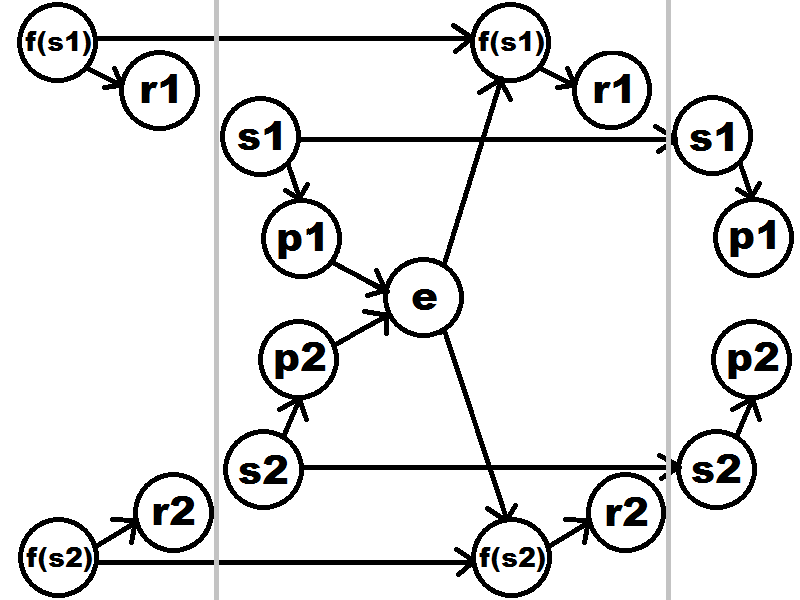
\includegraphics[scale=0.35]{../images/HMMlabeled.png} \end{center}

In order to absorb $e$ into our posterior, a few approximations are in order. First, we assume the number of participants is so large that we are able to compute the performances exactly. Mathematically, this means $\Pr(e \mid p_i)$ is proportional to a delta ``function" concentrated at the correct value of $p_i$. Hence, using Bayes' rule again,

\begin{align*}
f(s_i\mid e)
&\propto f(s_i)\Pr(e\mid s_i)
\\&= f(s_i)\int \Pr(e\mid p_i)f(p_i\mid s_i)\,dp_i
\\&\propto f(s_i)f(p_i\mid s_i)
\end{align*}

where the constants of proportionality depend on $e$ but not on $s_i$.

This suggests a natural two-phase update algorithm for each player $i$. In phase one, we estimate the MAP of $p_i$ given $e$. This estimate has very low error in the limit of very many participants, so we can take the MAP of $p_i$ to be its true value. In phase two, we update the posterior according to the above expression, and compute the new rating $r_i$ as the MAP of $s_i$ given $e$.

Note that, since the $p_i$ are assumed to be computed exactly, there is never a reason to retroactively update past estimates of performance. It follows that a round's non-participating players have posterior skill distribution identical to their prior; in particular, their ratings do not change.
\section{Skill estimation in two phases}
\label{sec:main-alg}
    \subsection{Performance estimation}
\label{sec:performance}

In this section, we describe the first phase of Elo-MMR. For notational convenience, we assume all probability expressions to be conditioned on the \textbf{prior context} $P_{i,< t}$, and omit the subscript $t$.

Our prior belief on each player's skill $S_i$ implies a prior distribution on $P_i$. Let's denote its probability density function (pdf) by
\begin{equation}
\label{eq:perf-prior} 
f_i(p) := \Pr(P_i = p) = \int \pi_i(s) \Pr(P_i = p \mid S_i=s) \,\mathrm{d}s,
\end{equation}
where $\pi_i(s)$ was defined in \Cref{eq:pi-s}. Let
\[F_i(p) := \Pr(P_i\le p) = \int_{-\infty}^p f_i(x) \,\dx,\]
be the corresponding cumulative distribution function (cdf). For the purpose of analysis, we'll also define the following ``loss'', ``draw'', and ``victory'' functions:
\begin{align*}
l_i(p) &:= \ddp\ln(1-F_i(p)) = \frac{-f_i(p)}{1 - F_i(p)},
\\d_i(p) &:= \ddp\ln f_i(p) = \frac{f'_i(p)}{f_i(p)},
\\v_i(p) &:= \ddp\ln F_i(p) = \frac{f_i(p)}{F_i(p)}.
\end{align*}

Evidently, $l_i(p) < 0 < v_i(p)$. Now we define what it means for the deviation $P_i - S_i$ to be log-concave.
\begin{definition}
\label{def:log-concave}
An absolutely continuous random variable on a convex domain is \textbf{log-concave} if its probability density function $f$ is positive on its domain and satisfies
\[f(\theta x + (1-\theta) y) > f(x)^\theta f(y)^{1-\theta},\;\forall\theta\in(0,1),x\neq y.\]
\end{definition}

Log-concave distributions appear widely, and include the Gaussian and logistic distributions used in Glicko, TrueSkill, and many others. We'll see inductively that our prior $\pi_i$ is log-concave at every round. Since log-concave densities are closed under convolution~\cite{concave}, the independent sum $P_i=S_i+(P_i-S_i)$ is also log-concave. Log-concavity is made very convenient by the following lemma, proved in the extended version of this paper:
\begin{lemma}
\label{lem:decrease}
If $f_i$ is continuously differentiable and log-concave, then the functions $l_i,d_i,v_i$ are continuous, strictly decreasing, and
\[l_i(p) < d_i(p) < v_i(p) \text{ for all }p.\]
\end{lemma}

For the remainder of this section, we fix the analysis with respect to some player $i$. As argued in \Cref{sec:bayes_model}, $P_i$ concentrates very narrowly in the posterior. Hence, we can estimate $P_i$ by its MAP, choosing $p$ so as to maximize:
\[\Pr(P_i=p\mid E^L_i,E^W_i) \propto f_i(p) \Pr(E^L_i,E^W_i\mid P_i=p).\]

Define $j\succ i$, $j\prec i$, $j\sim i$ as shorthand for $j\in E^L_i$, $j\in E^W_i$, $j\in \mathcal P\setminus (E^L_i\cup E^W_i)$ (that is, $P_j>P_i$, $P_j<P_i$, $P_j=P_i$), respectively. The following theorem yields our MAP estimate:
\begin{theorem}
\label{thm:uniq-max}
Suppose that for all $j$, $f_j$ is continuously differentiable and log-concave. Then the unique maximizer of $\Pr(P_i=p\mid E^L_i,E^W_i)$ is given by the unique zero of
\[Q_i(p) := \sum_{j \succ i} l_j(p) + \sum_{j \sim i} d_j(p) + \sum_{j \prec i} v_j(p).\]
\end{theorem}
The proof appears in the extended version of this paper. Intuitively, we're saying that the performance is the balance point between appropriately weighted wins, draws, and losses. Let's look at two specializations of our general model, to serve as running examples in this paper.

\paragraph{Gaussian performance model}
If both $S_j$ and $P_j-S_j$ are assumed to be Gaussian with known means and variances, then their independent sum $P_j$ will also be a known Gaussian. It is analytic and log-concave, so \Cref{thm:uniq-max} applies.

We substitute the well-known Gaussian pdf and cdf for $f_j$ and $F_j$, respectively. A simple binary search, or faster numerical techniques such as the Illinois algorithm or Newton's method, can be employed to solve for the unique zero of $Q_i$.

\begin{figure}
    \centering
    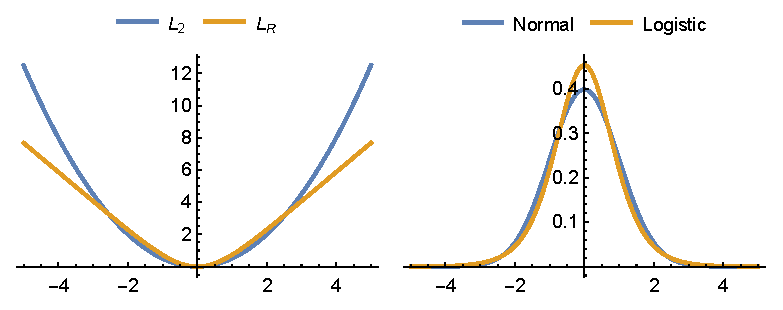
\includegraphics[width=1.05\columnwidth]{images/l2-lr-plot.eps}
    \caption{$L_2$ versus $L_R$ for typical values (left). Gaussian versus logistic probability density functions (right).}
    \label{fig:l2-lr-plot}
\end{figure}

\paragraph{Logistic performance model}
Now we assume the performance deviation $P_j-S_j$ has a logistic distribution with mean 0 and variance $\beta^2$. In general, the rating system administrator is free to set $\beta$ differently for each contest. Since shorter contests tend to be more variable, one reasonable choice might be to make $1/\beta^2$ proportional to the contest duration.

Given the mean and variance of the skill prior, the independent sum $P_j = S_j + (P_j-S_j)$ would have the same mean, and a variance that's increased by $\beta^2$. Unfortunately, we'll see that the logistic performance model implies a form of skill prior from which it's tough to extract a mean and variance. Even if we could, the sum does not yield a simple distribution.

For experienced players, we expect $S_j$ to contribute much less variance than $P_j-S_j$; thus, in our heuristic approximation, we take $P_j$ to have the same form of distribution as the latter. That is, we take $P_j$ to be logistic, centered at the prior rating $\mu^\pi_j = \argmax \pi_j$, with variance $\delta_j^2 = \sigma_j^2 + \beta^2$, where $\sigma_j$ will be given by \Cref{eq:variance}. This distribution is analytic and log-concave, so the same methods based on \Cref{thm:uniq-max} apply. 
Define the scale parameter $\bar\delta_j := \frac{\sqrt{3}}{\pi} \delta_j$. A logistic distribution with variance $\delta_j^2$ has cdf and pdf:
\begin{align*}
F_j(x) &= \frac { 1 } { 1 + e^{-(x-\mu^\pi_j)/\bar\delta_j} }
= \frac 12 \left(1 + \tanh\frac{x-\mu^\pi_j}{2\bar\delta_j} \right),
\\f_j(x) &= \frac { e^{(x-\mu^\pi_j)/\bar\delta_j} } { \bar\delta_j\left( 1 + e^{(x-\mu^\pi_j)/\bar\delta_j} \right)^2}
= \frac { 1 } { 4\bar\delta_j} \sech^2\frac{x-\mu^\pi_j}{2\bar\delta_j}.
\end{align*}

The logistic distribution satisfies two very convenient relations:
\begin{align*}
F'_j(x) = f_j(x) &= F_j(x) (1 - F_j(x)) / \bar\delta_j,
\\f'_j(x) &= f_j(x) (1 - 2F_j(x)) / \bar\delta_j,
\end{align*}
from which it follows that
\[d_j(p)
= \frac{1 - 2F_j(p)}{\bar\delta}
= \frac{-F_j(p)}{\bar\delta} + \frac{1 - F_j(p)}{\bar\delta}
= l_j(p) + v_j(p).\]

In other words, a tie counts as the sum of a win and a loss. This can be compared to the approach (used in Elo, Glicko, BAR, Topcoder, and Codeforces) of treating each tie as half a win plus half a loss.\footnote{Elo-MMR, too, can be modified to split ties into half win plus half loss. It's easy to check that \Cref{lem:decrease} still holds if $d_j(p)$ is replaced by
$w_l l_j(p) + w_v v_j(p)$
for some $w_l,w_v\in [0,1]$ with $|w_l-w_v|<1$.
In particular, we can set $w_l=w_v=0.5$. The results in \Cref{sec:properties} won't be altered by this change.}

Finally, putting everything together:
\[Q_i(p) = \sum_{j \succeq i} l_j(p) + \sum_{j \preceq i} v_j(p)
= \sum_{j \succeq i} \frac{-F_j(p)}{\bar\delta_j} + \sum_{j \preceq i} \frac{1 - F_j(p)}{\bar\delta_j}.\]
Our estimate for $P_i$ is the zero of this expression. The terms on the right correspond to probabilities of winning and losing against each player $j$, weighted by $1/\bar\delta_j$. Accordingly, we can interpret $\sum_{j\in \cP} (1-F_j(p))/\bar\delta_j$ as a weighted expected rank of a player whose performance is $p$. Similar to the performance computations in Codeforces and Topcoder, $P_i$ can thus be viewed as the performance level at which one's expected rank would equal $i$'s actual rank.


    

\section{Belief Update}

With $p_i$ in hand, we are ready for the second phase of the update! Recall that we seek to maximize

\[f(s_i\mid e) \propto f(s_i)f(p_i\mid s_i)\]

Ignoring for now the distinction between the posterior at round $t-1$ and the prior at round $t$ (we'll come back to this in the next section), we see that each round multiplies our belief p.d.f. by a logistic factor and a normalizing constant. Thus, our belief will always consist of a product of p.d.f.s.

Let's be a tad more general here and allow the belief to be any normalized product of normal and logistic p.d.f.s. The normal p.d.f.s can be composed into a single normal with mean and variance $(\mu_0, \tau_0^2)$. Let $R_i$ be the set of rounds in which player $i$ has participated, each contributing a logistic factor with parameters $(\mu_k, \tau_k^2)$ for $k\in R_i\cap \{1,\ldots,t\}$. Naturally, the new factor from round $t$ will have $\mu_t = p_{i,t}$ and $\tau_t = \gamma_{i,t}$. The other factors also satisfy $\mu_k = p_{i,k}$ but, as we'll see in the next section, $\tau_k$ increases with time and will exceed $\gamma_{i,k}$ in general. Again defining $\bar\tau_k = \frac{\sqrt{12}}{\pi} \tau_k$,

\[
f(s_i\mid e)
\propto e^{-(s_i-\mu_0)^2/\tau_0^2} \prod_{k\ge 1} \frac { 1 } { \cosh^2\frac{s_i-\mu_k} {\bar\tau_k} }
\]

Hence, there exists a constant $C$ such that

\[C - \frac 1 2 \ln f(s_i \mid e) = \frac{(s_i-\mu_0)^2}{2\tau_0^2} + \sum_{k\ge 1} \ln\left( \cosh\frac{s_i-\mu_k}{\bar\tau_k} \right)\]

Maximizing $f(s_i\mid e)$ amounts to minimizing this expression, so let's differentiate it w.r.t. $s_i$ and set the result to zero:

\[
0 = \frac{s_i-\mu_0}{\tau_0^2} + \sum_{k\ge 1} \frac{1}{\bar\tau_k} \tanh \frac {s_i-\mu_k} {\bar\tau_k}
\]

Similar to the performance computation in the previous section, here we have a monotonic function of $s_i$. To compute the post-round rating $r_i = \arg\max_{s_i} f(s_i \mid e)$, we may use binary search or Newton's method.

This time, the intuitive interpretation comes from the minimization objective that we differentiated. It has one term corresponding to each p.d.f. factor. The normal p.d.f. becomes a familiar $L^2$ penalty that pushes $s_i$ towards $\mu_0$. The logistic p.d.f.s are more interesting: they too become penalties that push $s_i$ towards $\mu_k$; however, instead of a simple squared error, each of these terms is a logarithm of a hyperbolic cosine!

At small scales (that is, when $|s_i-\mu_k| \ll \tau_k$), it acts like an $L^2$ penalty. However, at large scales (when $|s_i-\mu_k| \gg \tau_k$), it acts like an $L^1$ penalty! It's well-known that minimizing a sum of $L^2$ terms pushes the argument towards a weighted mean, while minimizing a sum of $L^1$ terms pushes the argument towards a weighted median.

The net result of these penalties is that $r_i$ acts like a mean of the historical performances $\mu_k = p_{i,k}$: it's easily checked that

\[r_i = \frac{\sum_k w_k\mu_k}{\sum_k w_k} \text{ where } w_0 = \frac{1}{\tau_0^2} \text{ and }
w_k = \frac{1}{\bar\tau_k(r_i-\mu_k)}\tanh\frac{r_i-\mu_k}{\bar\tau_k} \text{ for }k\ge 1.\]

$w_k$ is close to $1/\bar\tau_k^2$ for typical performances but vanishes for extreme outliers, making our rating algorithm robust to performances that are far below or above the usual. This robustness is due to the thicker tails of the logistic distribution, compared to the normal. Empirically, contest performances have indeed been seen to have thick tails, more like the logistic than the normal (TODO citation).

Note that when the weights are fixed, as in the $L^2$ case, it's possible to compute the posterior rating as a function of only the prior rating, prior weight, and the current round's performance and weight. This is no longer possible when using $L^1$ or $\ln\cosh$ penalties. Naively, it appears this method must remember the entire history of past performances: certainly, the latest rating alone is insufficient.

Luckily, it's possible to sustain negligible loss of precision while retaining only a bounded history length per player, thus keeping the time and memory overhead to within a constant factor. The exact means by which this is achieved depends on the noising method used, a matter we'll discuss later. For now, note that the $\tanh$ function behaves like the identity in the limit of large $\tau_k$. Hence, logistic factors with sufficiently large $\tau_k$ will come to resemble normal factors, which combine nicely.

As a final matter, we estimate the variance $\sigma_i^2$ of the posterior distribution on $s_i$. While this is intractable for general products of p.d.f.s, we take advantage of our observation that logistic factors behave in the limit like normal factors. Thus, we make an approximation based on a formula that holds for products of normal p.d.f.s:

\[\frac{1}{\bar\sigma_i^2} = \frac{1}{\tau_0^2} + \sum_k \frac{1}{\bar\tau_k^2}\]
    %\subsection{Initial Skill Distributions}

%\paul{Does our system preserve the mean rating of the population?}

%\aram{No it doesn't. Should this section be here? The newbie prior is not the only thing subject to hyperparameter search.}

%In our two-phase algorithm, skill distributions can be updated from round to round via \Cref{alg:update}. However, new players to the rating system must be initialized with an initial skill distribution. In practice, any initial distribution converges after the player participates in a few rounds. Thus, one approach is to seed the rating system with an initial pool of players from which an initial skill distribution can be estimated after a few rounds of play. Another approach is a simple hyper-parameter search over the initial skill distribution that optimizes for the prediction accuracy. In our experiments, we take the latter approach.
\section{Skill evolution over time}
\label{sec:skill-drift}
%This is an important component in applications, as players often train and improve between rounds.\footnote{This skill drift is modelled by almost all of the systems described in the introduction.} The time-varying skill is typically modelled by Gaussian noise, as we describe in \Cref{sec:skill-drift}.

Factors such as training and resting will change a player's skill over time. If we model skill as a static variable, our system will eventually grow so confident in its estimate that it will refuse to admit substantial changes. To remedy this, we introduce a skill evolution model, so that in general $S_t \neq S_{t'}$ for $t \neq t'$. Now rather than simply being equal to the previous round's posterior, the skill prior at round $t$ is given by
\begin{equation}
\label{eq:drift}
\pi_t(s) = \int \Pr(S_t = s \mid S_{t-1} = x) \Pr(S_{t-1} = x \mid P_{<t}) \,\dx.
\end{equation}

The factors in the integrand are the skill evolution model and the previous round's posterior, respectively. Following other Bayesian rating systems (e.g., Glicko, Glicko-2, and TrueSkill~\cite{G99, G12, HMG06}), we model the skill diffusions $S_t-S_{t-1}$ as independent zero-mean Gaussians. That is, $\Pr(S_t \mid S_{t-1}=x)$ is a Gaussian with mean $x$ and some variance $\gamma_t^2$. The Glicko system sets $\gamma_t^2$ proportionally to the time elapsed since the last update, corresponding to a continuous Brownian motion. Codeforces and Topcoder simply set $\gamma_t$ to a constant when a player participates, and zero otherwise, corresponding to changes that are in proportion to how often the player competes. Now we are ready to complete the two specializations of our rating system.

\paragraph{Gaussian performance model}
If both the prior and performance distributions at round $t-1$ are Gaussian, then the posterior is also Gaussian. Adding an independent Gaussian diffusion to our posterior on $S_{t-1}$ yields a Gaussian prior on $S_t$. By induction, the skill belief distribution forever remains Gaussian. This Gaussian specialization of the Elo-MMR framework lacks the R for robustness (see \Cref{thm:robust}), so we call it Elo-MM$\chi$.

\paragraph{Logistic performance model}
After a player's first contest round, the posterior in \Cref{eq:posterior} becomes non-Gaussian, rendering the integral in \Cref{eq:drift} intractable.

A very simple approach would be to replace the full posterior in \Cref{eq:posterior} by a Gaussian approximation with mean $\mu_t$ (equal to the posterior MAP) and variance $\sigma_t^2$ (given by \Cref{eq:variance}). As in the previous case, applying diffusions in the Gaussian setting is a simple matter of adding means and variances.

With this approximation, no memory is kept of the individual performances $P_t$. Priors are simply Gaussian, while posterior densities are the product of two factors: the Gaussian prior, and a logistic factor corresponding to the latest performance. To ensure robustness (see \Cref{sec:robust}), $\mu_t$ is computed as the argmax of this posterior \emph{before} replacement by its Gaussian approximation. We call the rating system that takes this approach Elo-MMR($\infty$).

As the name implies, it turns out to be a special case of Elo-MMR($\rho$). In the general setting with $\rho \in [0,\infty)$, we keep the full posterior from \Cref{eq:posterior}. Since we cannot tractably compute the effect of a Gaussian diffusion, we seek a heuristic derivation of the next round's prior, retaining a form similar to \Cref{eq:posterior} while satisfying many of the same properties as the intended diffusion.

\subsection{Desirable properties of a ``pseudodiffusion''}
\label{sec:desirable-props}
We begin by listing some properties that our skill evolution algorithm, henceforth called a ``pseudodiffusion'', should satisfy. The first two properties are natural:
\begin{itemize}[leftmargin=*]
\item \emph{Incentive-compatibility.} First and foremost, the pseudodiffusion must not break the incentive-compatibility of our rating system. That is, a rating-maximizing player should never be motivated to lose on purpose. (\Cref{thm:mono}).
\item \emph{Rating preservation.} The pseudodiffusion must not alter the $\argmax$ of the belief density. That is, the rating of a player should not change: $\mu^\pi_t = \mu_{t-1}$.
\end{itemize}
In addition, we borrow four properties of Gaussian diffusions:
\begin{itemize}[leftmargin=*]
\item \emph{Correct magnitude.} Pseudodiffusion with parameter $\gamma^2$ must increase the skill uncertainty, as measured by \Cref{eq:variance}, by $\gamma^2$.
\item \emph{Composability.} Two pseudodiffusions applied in sequence, first with parameter $\gamma_1^2$ and then with $\gamma_2^2$, must have the same effect as a single pseudodiffusion with parameter $\gamma_1^2 + \gamma_2^2$.
\item \emph{Zero diffusion.} In the limit as $\gamma \rightarrow 0$, the effect of pseudodiffusion must vanish, i.e., not alter the belief distribution.
\item \emph{Zero uncertainty.} In the limit as $\sigma_{t-1}\rightarrow 0$ (i.e., when the previous rating $\mu_{t-1}$ is a perfect estimate of $S_{t-1}$), our belief on $S_t$ must become Gaussian with mean $\mu_{t-1}$ and variance $\gamma^2$. Finer-grained information regarding the prior history $P_{\le t}$ must be erased.
\end{itemize}
In particular, Elo-MMR($\infty$) fails the \emph{zero diffusion} property because it simplifies the belief distribution, even when $\gamma=0$. In the proof of \Cref{thm:diffuse-prop}, we'll see that Elo-MMR($0$) fails the \emph{zero uncertainty} property. Thus, it is in fact necessary to have $\rho$ strictly positive and finite. In \Cref{sec:robust}, we'll come to interpret $\rho$ as a kind of inverse momentum.

\subsection{A heuristic pseudodiffusion algorithm}
\label{sec:pseudodiffusion}
Each factor in the posterior (see \Cref{eq:posterior}) has a parameter $\beta_k$. Define a factor's \textbf{weight} to be $w_k := 1/\beta_k^2$, which by \Cref{eq:variance} contributes to the \textbf{total weight} $\sum_k w_k=1/\sigma_t^2$. Here, unlike in \Cref{eq:average}, $w_k$ does not depend on $|\mu_t-p_k|$.

The approximation step of Elo-MMR($\infty$) replaces all the logistic factors by a single Gaussian whose variance is chosen to ensure that the total weight is preserved. In addition, its mean is chosen to preserve the player's rating, given by the unique zero of \Cref{eq:loss}. Finally, the diffusion step of Elo-MMR($\infty$) increases the Gaussian's variance, and hence the player's skill uncertainty, by $\gamma_t^2$; this corresponds to a decay in the weight.

To generalize the idea, we interleave the two steps in a continuous manner. The approximation step becomes a \textbf{transfer step}: rather than replace the logistic factors outright, we take away the same fraction from each of their weights, and \emph{place the sum of removed weights onto a new Gaussian factor}. In order for this operation to preserve ratings, the new factor must be centered at $\mu_{t-1}$. Since Gaussian pdfs compose, the prior Gaussian factor can be combined with the new one. The diffusion step becomes a \textbf{decay step}, reducing each factor's weight by the same fraction, chosen such that the overall uncertainty is increased by $\gamma_t^2$.

To make the idea precise, we generalize the posterior from \Cref{eq:posterior} with fractional \textbf{multiplicities} $\omega_k$; the $k$'th factor is raised to the power $\omega_k$. As a result, \Cref{eq:loss,eq:variance} become:
%initially set to $1$ for each $k\in\{0\}\cup\cH_t$. 
%The $k$'th factor is raised to the power $\omega_k$; in \Cref{eq:loss,eq:variance}, the corresponding term is multiplied by $\omega_k$.

\begin{align}
\label{eq:multiplicities}
L'(s) &= \frac{\omega_0(s-p_0)}{\beta_0^2} + \sum_{k\in\cH_t} \frac{\omega_k\pi}{\beta_k\sqrt{3}} \tanh \frac{(s-p_k)\pi}{\beta_k\sqrt{12}},\nonumber
\\\frac{1}{\sigma_t^2} &:= \sum_{k\in\{0\}\cup\cH_t}w_k,\quad\text{where }w_k := \frac{\omega_k}{\beta_k^2}.
\end{align}

For $\rho\in [0,\infty]$, the Elo-MMR($\rho$) algorithm continuously and simultaneously performs transfer and decay, with transfer proceeding at $\rho$ times the rate of decay. Holding $\beta_k$ fixed, changes to $\omega_k$ can be described in terms of changes to $w_k$:
\begin{align*}
\dot w_0 &= -r(t)w_0 + \rho r(t) \sum_{k\in\cH_t} w_k,
\\\dot w_k &= -(1+\rho)r(t)w_k \quad\text{for }k\in\cH_t,
\end{align*}
where the arbitrary decay rate $r(t)$ can be eliminated by a change of variable $\mathrm{d}\tau = r(t)\dt$. After some time $\Delta\tau$, the total weight will have decayed by a factor $\kappa := e^{-\Delta\tau}$, resulting in the new weights:
\begin{align*}
w_0^{new} &= \kappa w_0 + \left(\kappa-\kappa^{1+\rho}\right)\sum_{k\in\cH_t} w_k,
\\w_k^{new} &= \kappa^{1+\rho}w_k \quad\text{for }k\in\cH_t.
\end{align*}
In order for the uncertainty to increase from $\sigma_{t-1}^2$ to $\sigma_{t-1}^2+\gamma_t^2$, we must solve $\kappa/\sigma_{t-1}^2 = 1/(\sigma_{t-1}^2+\gamma_t^2)$ for the decay factor:
\[\kappa_t = \left(1 + \frac{\gamma_t^2}{\sigma_{t-1}^2}\right)^{-1}.\]

\setlength{\floatsep}{0pt}
\setlength{\textfloatsep}{1em}
\begin{algorithm}[t]
\caption{Elo-MMR($\rho,\beta, \gamma$)}
\label{alg:main}
\begin{algorithmic}
\FORALL{rounds $t$}
\FORALL{players $i\in\mathcal P_t$ in parallel}
\IF{$i$ has never competed before}
\STATE {$\mu_i, \sigma_i \gets \mu_{newcomer}, \sigma_{newcomer}$}
\STATE {$p_i, w_i \gets [\mu_i], [1/\sigma_i^2]$}
\ENDIF
%\STATE $\gamma \gets$ systemspecified()
\STATE diffuse($i,\gamma,\rho$)
\STATE $\mu^\pi_i, \delta_i \gets \mu_i,\sqrt{\sigma_i^2 + \beta^2}$
%\STATE Make $\mu^\pi_i,\delta_i$ accessible to all threads in the next loop
\ENDFOR
%\STATE $E \gets$ getevidence()
\FORALL{$i\in\mathcal P_t$ in parallel}
\STATE update($i,E_t,\beta$)
\ENDFOR
\ENDFOR
\end{algorithmic}
\end{algorithm}
\begin{algorithm}[t]
\caption{diffuse($i,\gamma,\rho$)}
\label{alg:diffuse}
\begin{algorithmic}
\STATE $\kappa \gets (1+\gamma^2/\sigma_i^2)^{-1}$
\STATE $w_G, w_L \gets \kappa^\rho w_{i,0}, (1-\kappa^\rho) \sum_{k\geq 0} w_{i,k}$
\STATE $p_{i,0} \gets (w_G p_{i,0} + w_L \mu_i) / (w_G+w_L)$
\STATE $w_{i,0} \gets \kappa (w_G+w_L)$
\FORALL{$k > 0$}
\STATE $w_{i,k} \gets \kappa^{1+\rho}w_{i,k}$
\ENDFOR
\STATE $\sigma_i \gets \sigma_i / \sqrt\kappa$
\end{algorithmic}
\end{algorithm}
\begin{algorithm}[t]
\caption{update($i,E,\beta$)}
\label{alg:update}
\begin{algorithmic}
\STATE $p \gets \mathrm{zero}_x\left(\sum_{j\preceq i}\frac{1}{\delta_j}\left( \tanh\frac {x - \mu^\pi_j} {2\bar\delta_j} - 1 \right) + \sum_{j\succeq i}\frac{1}{\delta_j}\left( \tanh\frac {x - \mu^\pi_j} {2\bar\delta_j} + 1 \right)\right)$
\STATE $p_i$.push($p$)
\STATE $w_i$.push($1/\beta^2$)
\STATE $\mu_i \gets \mathrm{zero}_x\left(w_{i,0}(x-p_{i,0}) + \sum_{k>0} \frac{w_{i,k}\beta^2}{\bar\beta} \tanh \frac {x-p_{i,k}} {2\bar\beta}\right)$
\end{algorithmic}
\end{algorithm}

\Cref{alg:main} details the full Elo-MMR($\rho$) rating system. The main loop runs whenever a round of competition takes place. First, new players are initialized with a Gaussian prior. Then, changes in player skill are modeled by \Cref{alg:diffuse}; note how the Gaussian prior is updated into a weighted combination with the newly created factor. Given the round rankings $E_t$, the first phase of \Cref{alg:update} solves an equation to estimate $P_t$. Finally, the second phase solves another equation for the rating $\mu_t$. 

The hyperparameters $\rho,\beta,\gamma$ are domain-dependent, and can be set by standard hyperparameter search techniques. For convenience, we assume $\beta$ and $\gamma$ are fixed and use the shorthand $\bar\beta_k := \frac{\sqrt{3}}{\pi} \beta_k$. Whereas our exposition used global round indices, here a subscript $k$ corresponds to the $k$'th round in player $i$'s participation history.

\begin{theorem}
\label{thm:diffuse-prop}
\Cref{alg:diffuse} with $\rho\in(0,\infty)$ meets all of the properties listed in \Cref{sec:desirable-props}.
\end{theorem}

\begin{proof}
We go through each of the six properties in order.
\begin{itemize}[leftmargin=*]
    \item \emph{Incentive-compatibility.} This property will be stated in \Cref{thm:mono}. To ensure that its proof carries through, the relevant facts to note here are that the pseudodiffusion algorithm ignores the performances $p_k$, and centers the transferred Gaussian weight at the rating $\mu_{t-1}$, which is trivially monotonic in $\mu_{t-1}$.
    \item \emph{Rating preservation.} Recall that the rating is the unique zero of $L'$ in \Cref{eq:multiplicities}. To see that this zero is preserved, note that the decay and transfer operations multiply $L'$ by constants ($\kappa_t$ and $\kappa_t^\rho$, respectively), before adding the new Gaussian term, whose contribution to $L'$ is zero at its center.
    \item \emph{Correct magnitude.} Follows from our derivation for $\kappa_t$.
    \item \emph{Composability.} Follows from \emph{correct magnitude} and the fact that every pseudodiffusion follows the same differential equations.
    \item \emph{Zero diffusion.} As $\gamma\rightarrow 0$, $\kappa_t\rightarrow 1$. Provided that $\rho<\infty$, we also have $\kappa_t^\rho\rightarrow 1$. Hence, for all $k\in\{0\}\cup\cH_t$, $w_k^{new} \rightarrow w_k$.
    \item \emph{Zero uncertainty.} As $\sigma_{t-1}\rightarrow 0$, $\kappa_t\rightarrow 0$. The total weight decays from $1/\sigma_{t-1}^2$ to $\gamma^2$. Provided that $\rho > 0$, we also have $\kappa_t^\rho\rightarrow 0$, so these weights transfer in their entirety, leaving behind a Gaussian with mean $\mu_{t-1}$, variance $\gamma^2$, and no additional history. \qedhere
\end{itemize}
\end{proof}



\section{Properties}

First, we discuss some properties that Elo-R has in common with the published systems of Codeforces and TopCoder, as well as the classics Elo and Glicko. All of these systems propagate belief changes forward in time, never backward. This approach is simple, efficient, and has the benefit of never retroactively changing ratings from the past, nor the ratings of player who are not actively competing. Elo-R and Glicko converge to the right results a bit faster than the others, by including an uncertainty parameter that starts high for new players.

The two-phase approach of Elo-R is a bit unique, in that it's not memoryless (unless the memory is set to merge all the way down to a length of 1). Rating changes depend not only on the current rating and uncertainty, but on a list of recent performance values. Thus, we cannot make the same guarantees as Codeforces \cite{Codeforces}. This is the price of a robust system: it's impossible to identify and eliminate outliers if we don't remember their values! Nevertheless, we have some analoguous guarantees:
\begin{itemize}
\item The rating is a monotonic function of the list of past performances. Thus, unlike on Topcoder \cite{forivsektheoretical}, a situation will never arise where we would wish to have scored less.
\item If you swap the order of two performances in the list, the rating goes up if the better performance moves forward in time, and down if the better performance moves backward. This follows from the fact that newer performances have smaller uncertainty, since uncertainties don't depend on the value of any performance.
\item The performance $p_i$ is measured in the same units as rating and has the property that, within a given contest, a higher ranking contestant always has higher $p_i$ than a lower ranking one. In case of ties, the contestant with higher rating $r_i$ also has (slightly) higher $p_i$.
\end{itemize}

The code and ratings of real Codeforces members as computed by Elo-R are available at https://github.com/EbTech/EloR. Original Codeforces ratings are at http://codeforces.com/ratings. One striking difference is massive inflation in the Codeforces system. Gennady Korotkevich, best known by his competitive programming handle ``tourist", has been the reigning world champion for years. Toward the end of 2011, his rating reached a new ceiling of about 2700 according to both systems. However, as of this writing, his rating on Elo-R has increased by about 300 additional points, while on Codeforces it increased by almost 900. To get a sense of the magnitude of this change, 900 points is the difference between an average member and a Grandmaster! Indeed, most of the variance in the Codeforces system is concentrated at the top, with much smaller rating differences between beginner and intermediate members. This is caused by certain ad hoc elements of the system that are not founded on any rigorous model.

This paper will not evaluate the predictive accuracy of Elo-R; my experience with it suggests it does better than the other local methods listed above, but it is possible to do better with global methods. It's difficult to do a fair evaluation because it's not clear what exactly some of these models are trying to predict, besides the qualitative assertion that players with higher ratings should win more often. For example, Elo-R might be judged on the log-likelihood of observed match results, according to its own belief model. However, the joint likelihood is difficult to compute, and many of the other systems lack a corresponding belief model. One reasonable approach would be to approximate the likelihood as we did when estimating $p_i$, and use cross-validation to optimize the parameters of each rating system according to this criterion. Such evaluations will remain open to future investigation. Instead, let's focus on a unique feature of Elo-R that's absent in the Codeforces system, and arguably in TopCoder as well.

\subsection{Analysis of Monotonicity}

This is a draft in progress. Constant factor noising satisfies monotonicity, but it appears the fancier method can break monotonicity in some extreme cases. The purpose of this analysis is to understand when that happens and if/how that should be fixed.

Let $f$ be a function of the form:

\[f(x) = \sum_{k=1}^n \frac{1}{\tau_k} \tanh \frac {x-\mu_k} {\tau_k}\]

Then $f$ is a strictly increasing function of $x$. Let $r$ be the unique point at which $f(r) = 0$. Similarly, define

\[g(x) = \sum_{k=1}^m \frac{1}{\sigma_k} \tanh \frac {x-\nu_k} {\sigma_k}\]

such that $g(x) \ge f(x)$ for all $x$. Then $g$ too is strictly increasing: let $s$ be the unique point at which $g(s) = 0$. We cannot have $s > r$, as that would imply $0 = g(s) \ge f(s) > f(r) = 0$. Hence, $s \le r$. Furthermore, $\sum_k \frac{1}{\tau_k} = \sum_k \frac{1}{\sigma_k}$ because

\[\sum_k \frac{1}{\tau_k}
= \lim_{x\rightarrow\infty} f(x)
\le \lim_{x\rightarrow\infty} g(x)
= \sum_k \frac{1}{\sigma_k}
= -\lim_{x\rightarrow -\infty} g(x)
\le -\lim_{x\rightarrow -\infty} f(x)
= \sum_k \frac{1}{\tau_k}\]

Let $\eta$ be the noising operation:

\[\eta[f](x) = \sum_k \frac{1}{\tau'_k} \tanh \frac {x-\mu_k} {\tau'_k}\]
\[\eta[g](x) = \sum_k \frac{1}{\sigma'_k} \tanh \frac {x-\nu_k} {\sigma'_k}\]

\[ \frac{\sum_k 1 / \tau'^2_k}{\sum_k 1 / \tau^2_k} = \frac{\sum_k 1 / \sigma'^2_k}{\sum_k 1 / \sigma^2_k} \]

\[\frac{1}{\tau'_k} \tanh \frac {r-\mu_k} {\tau'_k}
= \frac{1}{\kappa^2\tau_k} \tanh \frac {r-\mu_k} {\tau_k}\]

\[\frac{1}{\sigma'_k} \tanh \frac {s-\nu_k} {\sigma'_k}
= \frac{1}{\lambda^2\sigma_k} \tanh \frac {s-\nu_k} {\sigma_k}\]

where $\kappa,\lambda$ do not depend on the subscripts $k$. It's easy to see that $\eta[f]$ and $\eta[g]$, too, are strictly increasing, with the same zero as $f$ and $g$, respectively.

We want to show that $\eta[g](x) \ge \eta[f](x)$ for all $x$. From this it will follow, as it did with $f$ and $g$, that the unique zero of $\eta[g]$ is no larger than that of $\eta[f]$.

Proof: we start by summarizing some of the above facts:

\[ \eta[f](s) \le \eta[f](r) = 0 = \eta[g](s) \le \eta[g](r) \]

For contradiction, suppose $\eta[g](t) < \eta[f](t)$ for some $t$. If $t\in [s,r]$, then

\[ 0 = \eta[g](s) \le \eta[g](t) < \eta[f](t) \le \eta[f](r) = 0 \]

which is a contradiction. For the rest of the proof, we can suppose $t < s$, since symmetry then takes care of the $t > r$ case. Let's only look at points $t$ and $s$. So far we have:

\[ f(t) < f(s) \le g(s) \]

\[ f(t) \le g(t) < g(s) \]

\[ \eta[g](t) < \eta[f](t) < \eta[f](s) \le 0 = \eta[g](s) \]

\subsection{Noising Methods}

So far, I can think of four reasonable noising methods. TODO: make this section into a table, with smileys replaced by colors: :D to green, :) to yellow, :( to red.

\subsubsection{Normal Approximation}

After each rating update, replace the posterior (which is the now product of one normal p.d.f. and one logistic p.d.f.) with a normal approximation. Then simply add Gaussian noise. This is the only method that does not accumulate a product of many logistic p.d.f.s, one for each recent performance.

Human-interpretable formulas: yes :D

Rating is a Markov state: yes :D

Monotonic in past performances: yes :D

Noising preserves MAP skill: yes :D

Saved history length: zero :D

Persistent outlier deweighting: immediate freeze-in, weights relative to rating at inception :)

Consistent change accelerates movement: no, slow convergence :(

\subsubsection{Constant Multiple on only the leading $\tau$}

The $\tau$ inside the $\tanh$ doesn't change. In other words, while the weight on each logistic factor is reduced over time, its variance is unchanged, so it never approaches the normal limit.

Human-interpretable formulas: yes :D

Rating is a Markov state: no :(

Monotonic in past performances: yes :D

Noising preserves MAP skill: yes :D

Saved history length: high :(

Persistent outlier deweighting: no freeze-in, weights relative to current rating :)

Consistent change accelerates movement: yes :D

\subsubsection{Constant Multiple on all $\tau$}

All of the $\tau$ change.

Human-interpretable formulas: yes :D

Rating is a Markov state: no :(

Monotonic in past performances: yes :D

Noising preserves MAP skill: no :(

Saved history length: low :)

Persistent outlier deweighting: outlierness is eventually forgotten, full weight restored :(

Consistent change accelerates movement: somewhat :)

\subsubsection{Fancy Method}

This is my favorite method. Regrettably, it fails the monotonicity criterion.

Human-interpretable formulas: yes :D

Rating is a Markov state: no :(

Monotonic in past performances: no :(

Noising preserves MAP skill: yes :D

Saved history length: low :)

Persistent outlier deweighting: gradual freeze-in, weights relative to neighbors in time :D

Consistent change accelerates movement: yes :D

\subsection{Robustness}

Imagine a player who performs very consistently over a long period of time, repeatedly achieving $p_i = 1000$ until convergence. Now, perhaps as a result of attending an intensive training camp in Petrozavodsk, their skill changes dramatically. From this point on, they consistently achieve $p_i = 3000$.

How does each rating system respond to the first such surprise occurrence? Elo-R treats the new result as a fluke, an outlier that ought to be ignored. The player gains 48 points; as a result of the parameters we set, this is the maximum possible for an experienced player as $p_i \rightarrow \infty$. In practice, ratings may change by more than 48, as the maximum depends on existing fluctuations in their history; here we're looking at the extreme example of a player with a history of always performing at exactly $p_i = 1000$.

\begin{center} 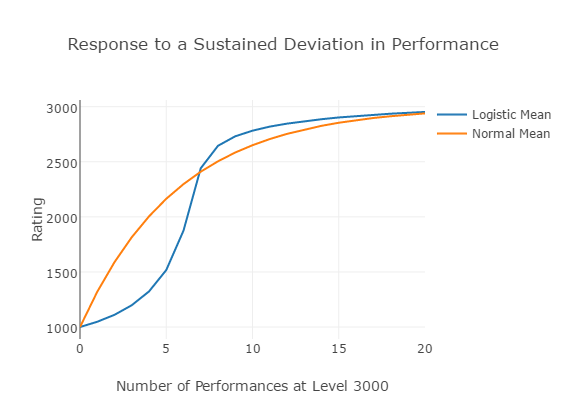
\includegraphics[scale=0.5]{../images/ResponsePlot.png} \end{center}

Had we tried to perform outlier reduction in a memoryless fashion, we would continue to increase the rating by 48 per match, oblivious to the possibility that the player truly did experience a sudden improvement. In Elo-R, the outlier status of a performance is treated as tentative. If later matches support the hypothesis of having improved, the rating will increase by an additional 63 points, followed by over 100 points in each of the third and following matches, as plotted by the blue curve above.

After six consecutive matches with $p_i = 3000$, the rating is 1875 and very unstable (even though $\sigma_i$ is unchanged!). The system is no longer sure which to trust: the extensive history at level 1000, or the smaller number of recent matches at level 3000. Depending on what comes next, the player's rating can very quickly fall toward 1000 or rise toward 3000. However, note that in either case, the change will not overshoot, say to 5000, unless enough new evidence is accumulated at that level. As the $p_i=3000$ streak continues, the seventh match on the blue curve jumps by a whopping 566 points. As the player's rating converges to 3000, the old $p_i = 1000$ data acquires outlier status, thus speeding convergence.

In contrast, while a system such as Codeforces does not compute $p_i$ values in quite in the same way, we can obtain a good approximation by removing outlier reduction from Elo-R, effectively treating the performances to be averaged as normal instead of logistic measurements. This makes the system effectively memoryless, since it turns out that each match simply moves the rating about 16\% closer to the new $p_i$ value, independent of the history. With this change, we obtain the orange curve, which jumps a whopping 320 points at the very first performance. Indeed, there is no limit: if you could find players whose ratings are extremely high, and beat them even once, your rating would take arbitrarily large leaps.

Note that this is not quite true of TopCoder, which incorporates a hack that caps the maximum rating change: if TopCoder's update formula demands too large a change, the cap kicks in. In contrast, Elo-R's cap is a natural and smooth consequence of its update formula and is sensitive to whether a change is charting new territory, or merely confirming a plausible hypothesis. TopCoder does attempt to make the magnitude of its updates sensitive to the amount of fluctuation in a player's history, using a volatility measure, but this measure does not account for the direction of the changes, resulting in the non-monotonicity flaw mentioned above.

Notwithstanding arguments that a high rating ought to properly be earned over multiple matches rather than a single fluke, the other danger is that these observations also hold in reverse: one bad day on Codeforces can seriously damage one's rating and negate several rounds of steady progress. By using heavy-tailed logistic distributions everywhere, Elo-R understands that unusually high or low performances do occasionally occur, and one round in isolation is never a reliable signal.

Interestingly, despite the slow start, the blue curve ultimately converges faster than the orange one. Since Elo-R uses its memory to dynamically adapt its view of potential outliers, it overtakes the orange curve as soon as new evidence outweighs the old hypothesis!

\subsection{Numerical analysis}

The ratings accumulate $O(\epsilon)$ numerical error per match, and likely a lot less in the long run due to statistical averaging...
\section{Experiments}
\label{sec:experiments}
In this section, we compare various rating systems on real-world datasets, mined from several sources that will be described in \Cref{sec:datasets}. The metrics are runtime and predictive accuracy, as described in \Cref{sec:metrics}. Implementations of all rating systems, dataset mining, and additional processing used in our experiments can be found at {\tt\url{https://github.com/EbTech/Elo-MMR}}.

We compare Elo-MM$\chi$ and Elo-MMR($\rho$) against the industry-tested rating systems of Codeforces and Topcoder. For a fairer comparison, we hand-coded efficient versions of all four algorithms in the safe subset of Rust, parellelized using the Rayon crate; as such, the Rust compiler verifies that they contain no data races~\cite{stone2017rayon}. Our implementation of Elo-MMR($\rho$) makes use of the optimizations in \Cref{sec:runtime}, bounding both the number of sampled opponents and the history length by 500. In addition, we test the improved TrueSkill algorithm of \cite{NS10}, basing our code on an open-source implementation of the same algorithm. The inherent seqentiality of its message-passing procedure prevented us from parallelizing it. All experiments were run on a 2.0 GHz 24-core Skylake machine with 24 GB of memory.

\paragraph{Hyperparameter search}
To ensure fair comparisons, we ran a separate grid search for each triple of algorithm, dataset, and metric, over all of the algorithm's hyperparameters. The hyperparameter set that performed best on the first 10\% of the dataset, was then used to test the algorithm on the remaining 90\% of the dataset. 

%We find that our rating performs slightly better than all competitors in terms of predictive power. In terms of computational time however, we show that Elo-MMR is up to an order of magnitude faster than Codeforces.

\subsection{Datasets}
\label{sec:datasets}

\begin{table}[t]
\begin{tabular}{l|l|l}
\hline
\textbf{Dataset} & \textbf{\# contests} & \textbf{avg. \# participants / contest} \\ \hline
Codeforces       & 1087                & 2999                                     \\ %\hline
Topcoder         & 2023                & 403                                   \\ %\hline
Reddit           & 1000                & 20                                       \\
%\hline
Synthetic        & 50                  & 2500     \\ \hline
\end{tabular}
    \caption{Summary of test datasets.}
    \label{tab:dataset-summary}
    \vspace{-1.2em}
\end{table}

Due to the scarcity of public domain datasets for rating systems, we mined three datasets to analyze the effectiveness of our system. The datasets were mined using data from each source website's inception up to October 9th, 2020. We also created a synthetic dataset to test our system's performance when the data generating process matches our theoretical model. Summary statistics of the datasets are presented in \Cref{tab:dataset-summary}.

\paragraph{Codeforces contest history}
This dataset contains the current entire history of rated contests ever run on codeforces.com, the dominant platform for online programming competitions. The Codeforces platform has over 850K users, over 300K of whom are rated, and has hosted over 1000 contests to date. Each contest has a couple thousand participants on average. A typical contest takes 2 to 3 hours and contains 5 to 8 problems. Players are ranked by total points, with more points typically awarded for tougher problems and for early solves. They may also attempt to ``hack'' one another's submissions for bonus points, identifying test cases that break their solutions. %The sheer number of highly motivated participants in these competitions, as well as their very accessible data API, made it the top choice for our explorations.
\looseness=-1

\paragraph{Topcoder contest history}
This dataset contains the current entire history of algorithm contests ever run on the topcoder.com. Topcoder is a predecessor to Codeforces, with over 1.4 million total users and a long history as a pioneering platform for programming contests. It hosts a variety of contest types, including over 2000 algorithm contests to date. The scoring system is similar to Codeforces, but its rounds are shorter: typically 75 minutes with 3 problems.

\paragraph{SubredditSimulator threads}
This dataset contains data scraped from the current top-1000 most upvoted threads on the website {\tt\url{reddit.com/r/SubredditSimulator/}}. Reddit is a social news aggregation website with over 300 million users. The site itself is broken down into sub-sites called subreddits. Users then post and comment to the subreddits, where the posts and comments receive votes from other users. In the subreddit SubredditSimulator, users are language generation bots trained on text from other subreddits. Automated posts are made by these bots to SubredditSimulator every 3 minutes, and real users of Reddit vote on the best bot. Each post (and its associated comments) can thus be interpreted as a round of competition between the bots who commented. 

\paragraph{Synthetic data}
This dataset contains 10K players, with skills and performances generated according to the Gaussian generative model in \Cref{sec:bayes_model}. Players' initial skills are drawn i.i.d. with mean $1500$ and variance $350^2$. Players compete in all rounds, and are ranked according to independent performances with variance $200^2$. Between rounds, we add i.i.d. Gaussian increments with variance $35^2$ to each of their skills.
% Uh is this the logistic or the Gaussian model??????

\subsection{Evaluation metrics}
\label{sec:metrics}
To compare the different algorithms, we define two measures of predictive accuracy. Each metric will be defined on individual contestants in each round, and then averaged:
\[\mathrm{\bf aggregate(metric)} := \frac{\sum_t \sum_{i\in\mathcal P_t} \mathrm{\bf metric}(i,t)}{\sum_t |\mathcal P_t|}.\]

\paragraph{Pair inversion metric~\cite{HMG06}}
Our first metric computes the fraction of opponents against whom our ratings predict the correct pairwise result, defined as the higher-rated player either winning or tying: 
\[\mathrm{\bf pair\_inversion}(i,t) := \frac{\text{\# correctly predicted matchups}}{|\mathcal P_t|-1} \times 100\%.\]
This metric was used in the original evaluation of TrueSkill~\cite{HMG06}.

\paragraph{Rank deviation}
Our second metric compares the rankings with the total ordering that would be obtained by sorting players according to their prior rating. The penalty is proportional to how much these ranks differ for player $i$:
\[\mathrm{\bf rank\_deviation}(i,t) := \frac{|\text{actual rank} - \text{predicted rank}|}{|\mathcal P_t|-1} \times 100\%.\]
In the event of ties, among the ranks within the tied range, we use the one that comes closest to the rating-based prediction.

% \paragraph{Entropy-based metric}
% For this metric, we evaluate the interpretability of the system ratings. As specified in \Cref{sec:bayes_model}, we assume player performances follow a Bradley-Terry model\paul{add BT and thurstone to this section}. In particular, we assume the probability of participants $i$ beating $j$ in a round $R$ is predicted by the simple formula \[\Pr[i \succ j] = \frac{1}{1 + 10^{\frac{\mu_i - \mu_j}{400}}}.\]
% As previously stated, this formula is assumed by the classic Elo rating system as well as the Codeforces rating system~\cite{...}, with the main benefit being that players can easily interpret the meaning of their ratings. To measure the interpretability, we measure the distance between the win distribution implied by the rating system and the actual win distribution. One way to do this is to measure the cross-entropy (which is equal to the KL-divergence up to an additive constant) via the follow formula:
% \[\mathrm{entropy} = -\frac{1}{\text{\# total pairs}} \sum_{\substack{i,j \in R \\ i \succ j}} \log \frac{1}{1 + 10^{\frac{\mu_i - \mu_j}{400}}}.\]

\subsection{Empirical results}
\begin{table*}
\begin{tabular}{l|ll|ll|ll|ll|ll}
 \hline
\multirow{2}{*}{\textbf{Dataset}} &
  \multicolumn{2}{l|}{\textbf{Codeforces}} &
  \multicolumn{2}{l|}{\textbf{Topcoder}} &
  \multicolumn{2}{l|}{\textbf{TrueSkill}} &
  \multicolumn{2}{l|}{\textbf{Elo-MM$\boldsymbol\chi$}} & 
  \multicolumn{2}{l}{\textbf{Elo-MMR($\boldsymbol\rho$)}} \\ \cline{2-11}
&
  pair inv. &
  rank dev. &
  pair inv. &
  rank dev. &
  pair inv. &
  rank dev. &
  pair inv. &
  rank dev. &
  pair inv. &
  rank dev. \\ \hline
Codeforces & 78.3\% & 14.9\% & 78.5\% & 15.1\% & 61.7\% & 25.4\% & 78.5\% & 14.8\% & {\bf 78.6}\% & {\bf 14.7}\% \\ %\hline
Topcoder  & 72.6\%     & 18.5\%     & 72.3\% & 18.7\%  & 68.7\% & 20.9\% & 73.0\% & 18.3\% & {\bf 73.1}\% & {\bf 18.2}\% \\ %\hline
Reddit     & 61.5\%     & 27.3\%     & 61.4\% & 27.4\% & 61.5\% & {\bf 27.2}\% & 61.6\% & 27.3\% & {\bf 61.6\%} & 27.3\% \\ %\hline
Synthetic  & {\bf 81.7\%}     & 12.9\%     & {\bf 81.7}\% & {\bf 12.8}\% & 81.3\% & 13.1\% & {\bf 81.7}\% & {\bf 12.8}\% & {\bf 81.7\%} & {\bf 12.8\%} \\ \hline
\end{tabular}
\caption{Performance of each rating system on the pairwise inversion and rank deviation metrics. Bolded entries denote the best performances (highest pair inv. or lowest rank dev.) on each metric and dataset.}
\label{tbl:metric-results}
\vspace{-1.2em}
\end{table*}

\begin{table}
\begin{tabular}{l|lllll}
\hline
\textbf{Dataset} & \textbf{CF} & \textbf{TC} & \textbf{TS} & \textbf{Elo-MM$\boldsymbol\chi$} & \textbf{Elo-MMR($\boldsymbol\rho$)} \\ \hline
Codeforces & 212.9 & 72.5 & 67.2 & {\bf 31.4} & 35.4\\
Topcoder   & 9.60 & {\bf 4.25} & 16.8 & 7.00 & 7.52\\
Reddit     & 1.19  & 1.14 & {\bf 0.44} & 1.14 & 1.42 \\
Synthetic  & 3.26  & 1.00 & 2.93 & {\bf 0.81} & 0.85 \\ \hline
\end{tabular}
\caption{Total compute time over entire dataset, in seconds.}
\label{tbl:time-results}
\vspace{-1.2em}
\end{table}

Recall that Elo-MM$\chi$ has a Gaussian performance model, matching the modeling assumptions of Topcoder and TrueSkill. Elo-MMR($\rho$), on the other hand, has a logistic performance model, matching the modeling assumptions of Codeforces and Glicko. While $\rho$ was included in the hyperparameter search, in practice we found that all values between $0$ and $1$ produce very similar results.

To ensure that errors due to the unknown skills of new players don't dominate our metrics, we excluded players who had competed in less than 5 total contests. In most of the datasets, this reduced the performance of our method relative to the others, as our method seems to converge more accurately. Despite this, we see in \Cref{tbl:metric-results} that both versions of Elo-MMR outperform the other rating systems in both the pairwise inversion metric and the ranking deviation metric.
\looseness=-1

We highlight a few key observations. First, significant performance gains are observed on the Codeforces and Topcoder datasets, despite these platforms' rating systems having been designed specifically for their needs. Our gains are smallest on the synthetic dataset, for which all algorithms perform similarly. This might be in part due to the close correspondence between the generative process and the assumptions of these rating systems. Furthermore, the synthetic players compete in all rounds, enabling the system to converge to near-optimal ratings for every player. Finally, the improved TrueSkill performed well below our expectations, despite our best efforts to improve it. We suspect that the message-passing numerics break down in contests with a large number of individual participants. The difficulties persisted in all TrueSkill implementations that we tried, including on Microsoft's popular {\tt Infer.NET} framework~\cite{InferNET18}. To our knowledge, we are the first to present experiments with TrueSkill on contests where the number of participants is in the hundreds or thousands. In preliminary experiments, TrueSkill and Elo-MMR score about equally when the number of ranks is less than about 60.

Now, we turn our attention to \Cref{tbl:time-results}, which showcases the computational efficiency of Elo-MMR. On smaller datasets, it performs comparably to the Codeforces and Topcoder algorithms. However, the latter suffer from a quadratic time dependency on the number of contestants; as a result, Elo-MMR outperforms them by almost an order of magnitude on the larger Codeforces dataset.

Finally, in comparisons between the two Elo-MMR variants, we note that while Elo-MMR($\rho$) is more accurate, Elo-MM$\chi$ is always faster. This has to do with the skill drift modeling described in \Cref{sec:skill-drift}, as every update in Elo-MMR($\rho$) must process $O(\log\frac 1\epsilon)$ terms of a player's competition history.

\section{Conclusions}
This paper introduces the Elo-MMR rating system, which is in part a generalization of the two-player Glicko system, allowing any number of players. By developing a Bayesian model and taking the limit as the number of participants goes to infinity, we obtained simple, human-interpretable rating update formulas. Furthermore, we saw that the algorithm is incentive-compatible, robust to extreme performances, asymptotically fast, and embarrassingly parallel. To our knowledge, our system is the first to rigorously prove all these properties in a setting with more than two individually ranked players. In terms of practical performance, we saw that it outperforms existing industry systems in both prediction accuracy and computation speed.
%In particular, we compare against the popular CodeForces, Topcoder, and TrueSkill rating systems, which are deployed on platforms with hundreds of thousands to millions of users.

This work can be extended in several directions. First, the choices we made in modeling ties, pseudodiffusions, and opponent subsampling are by no means the only possibilities consistent with our Bayesian model of skills and performances. Second, it may be possible to further improve accuracy by fitting more flexible performance and skill evolution models to application-specific data.

Another useful extension would be to team competitions. Given a performance model for teams, Elo-MMR infers each team's performance. To make this useful in settings where teams are frequently reassigned, we must model teams in terms of their individual members; unfortunately, it's not possible to precisely infer an individual's performance from team rankings alone. Therefore, it becomes necessary to condition an individual's skill on their team's performance. In the case where a team's performance is modeled as the sum of its members' independent Gaussian contributions, elementary facts about multivariate Gaussian distributions enable posterior skill inferences at the individual level. Generalizing this approach to other models remains an open challenge.

% Probably redundant: The algorithm itself is trivially parallelizable, and further speedup can be attained through a simple sub-sampling strategy. We believe there is potential to improve the performance even more, either through a more sophisticated sub-sampling strategy, interpolation, or by combining our two-phase approach with a factor graph framework similar to that of TrueSkill~\cite{HMG06, KFL01}. 

Over the past decade, online competition communities such as Codeforces have grown exponentially. As such, considerable work has gone into engineering scalable and reliable rating systems. Unfortunately, many of these systems have not been rigorously analyzed in the academic community. We hope that our paper and open-source release will open new explorations in this area.

%In addition, we invite non-technical sporting communities, such as the Spartan Race and DanceSport, to find uses of our skill estimation package.

% IMPORTANT: This conference is double blind, which (aside from anonymous authors) means that we cannot post links to our git or have acknowledgements.

\section*{Acknowledgements}
The authors are indebted to Daniel Sleator and Danica J. Sutherland for initial discussions that helped inspire this work, and to Nikita Gaevoy for the open-source improved TrueSkill upon which our implementation is based. Experiments in this paper are funded by a Google Cloud Research Grant. The second author is supported by a VMWare Fellowship and the Natural Sciences and Engineering Research Council of Canada.

\balance

%\appendix
% \section*{Appendix}
\begingroup
\def\thetheorem{\ref{lem:decrease}}
\begin{lemma}
If $f_i$ is continuously differentiable and log-concave, then the functions $l_i,d_i,v_i$ are continuous, strictly decreasing, and
\[l_i(p) < d_i(p) < v_i(p) \text{ for all }p.\]
\end{lemma}
\addtocounter{theorem}{-1}
\endgroup
\begin{proof}
Continuity of $F_i,f_i,f'_i$ implies that of $l_i,d_i,v_i$. It's known~\cite{concave} that log-concavity of $f_i$ implies log-concavity of both $F_i$ and $1-F_i$. As a result, $l_i$, $d_i$, and $v_i$ are derivatives of strictly concave functions; therefore, they are strictly decreasing. In particular, each of

\[v'_i(p) = \frac{f'_i(p)}{F_i(p)} - \frac{f_i(p)^2}{F_i(p)^2},\quad
l'_i(p) = \frac{-f'_i(p)}{1-F_i(p)} - \frac{f_i(p)^2}{(1-F_i(p))^2},\]

are negative for all $p$, so we conclude that

\begin{align*}
d_i(p) - v_i(p)
= \frac{f'_i(p)}{f_i(p)} - \frac{f_i(p)}{F_i(p)}
&= \frac{F_i(p)}{f_i(p)} v'_i(p)
< 0,
\\l_i(p) - d_i(p)
= -\frac{f'_i(p)}{f_i(p)} -\frac{f_i(p)}{1-F_i(p)}
&= \frac{1-F_i(p)}{f_i(p)} l'_i(p)
< 0.
\end{align*}

\end{proof}

\begingroup
\def\thetheorem{\ref{thm:uniq-max}}
\begin{theorem}
Suppose that for all $j$, $f_j$ is continuously differentiable and log-concave. Then the unique maximizer of $\Pr(P_i=p\mid E^L_i,E^W_i)$ is given by the unique zero of
\[Q_i(p) = \sum_{j \succ i} l_j(p) + \sum_{j \sim i} d_j(p) + \sum_{j \prec i} v_j(p).\]
\end{theorem}
\addtocounter{theorem}{-1}
\endgroup

\begin{proof}
First, we rank the players by their buckets according to $\floor{P_j/\epsilon}$, and take the limiting probabilities as $\epsilon\rightarrow 0$:
\begin{align*}
    \Pr(\floor{\frac{P_j}\epsilon} > \floor{\frac{p}\epsilon})
    &= \Pr(p_j \ge \epsilon\floor{\frac{p}\epsilon} + \epsilon)
    \\&= 1 - F_j(\epsilon\floor{\frac{p}\epsilon} + \epsilon)
    \rightarrow 1 - F_j(p),
    \\\Pr(\floor{\frac{P_j}\epsilon} < \floor{\frac{p}\epsilon})
    &= \Pr(p_j < \epsilon\floor{\frac{p}\epsilon})
    \\&= F_j(\epsilon\floor{\frac{p}\epsilon})
    \rightarrow F_j(p),
    \\\frac 1\epsilon \Pr(\floor{\frac{P_j}\epsilon} = \floor{\frac{p}\epsilon})
    &= \frac 1\epsilon \Pr(\epsilon\floor{\frac{p}\epsilon} \le P_j < \epsilon\floor{\frac{p}\epsilon} + \epsilon)
    \\&= \frac 1\epsilon\left( F_j(\epsilon\floor{\frac{p}\epsilon} + \epsilon) - F_j(\epsilon\floor{\frac{p}\epsilon}) \right)
    \rightarrow f_j(p).
\end{align*}

Let $L_{jp}^\epsilon$, $W_{jp}^\epsilon$, and $D_{jp}^\epsilon$ be shorthand for the events $\floor{\frac{P_j}\epsilon} > \floor{\frac{p}\epsilon}$, $\floor{\frac{P_j}\epsilon} < \floor{\frac{p}\epsilon}$, and $\floor{\frac{P_j}\epsilon} = \floor{\frac{p}\epsilon}$. respectively. These correspond to a player who performs at $p$ losing, winning, and drawing against $j$, respectively, when outcomes are determined by $\epsilon$-buckets. Then,
\begin{align*}
\Pr(E^W_i,E^L_i\mid P_i=p)
&= \lim_{\epsilon\rightarrow 0}
\prod_{j \succ i} \Pr(L_{jp}^\epsilon)
\prod_{j \prec i} \Pr(W_{jp}^\epsilon)
\prod_{j \sim i, j\ne i} \frac{\Pr(D_{jp}^\epsilon)}\epsilon
\\&= \prod_{j \succ i} (1 - F_j(p)) \prod_{j \prec i} F_j(p) \prod_{j \sim i, j\ne i} f_j(p),
\\\Pr(P_i=p \mid E^L_i,E^W_i)
&\propto f_i(p) \Pr(E^L_i,E^W_i\mid P_i=p)
\\&= \prod_{j \succ i} (1 - F_j(p)) \prod_{j \prec i} F_j(p) \prod_{j \sim i} f_j(p),
\\\ddp\ln \Pr(P_i=p \mid E^L_i,& E^W_i) = \sum_{j \succ i} l_j(p) + \sum_{j \prec i} v_j(p) + \sum_{j \sim i} d_j(p) = Q_i(p).
\end{align*}

Since \Cref{lem:decrease} tells us that $Q_i$ is strictly decreasing, it only remains to show that it has a zero. If the zero exists, it must be unique and it will be the unique maximum of $\Pr(P_i=p \mid E^L_i,E^W_i)$.

To start, we want to prove the existence of $p^*$ such that $Q_i(p^*) < 0$. Note that it's not possible to have $f'_j(p) \ge 0$ for all $p$, as in that case the density would integrate to either zero or infinity. Thus, for each $j$ such that $j\sim i$, we can choose $p_j$ such that $f'_j(p_j) < 0$, and so $d_j(p_j) < 0$. Let $\alpha = -\sum_{j\sim i} d_j(p_j) > 0$.

Let $n = |\{j:\,j \prec i\}|$. For each $j$ such that $j \prec i$, since $\lim_{p\rightarrow\infty}v_j(p) = 0/1 = 0$, we can choose $p_j$ such that $v_j(p_j) < \alpha/n$. Let $p^* = \max_{j\preceq i} p_j$. Then,
\[
\sum_{j \succ i} l_j(p^*) \le 0, \quad \sum_{j \sim i} d_j(p^*) \le -\alpha, \quad \sum_{j \prec i} v_j(p^*) < \alpha.
\]

Therefore,
\begin{align*}
Q_i(p^*)
&= \sum_{j \succ i} l_j(p^*) + \sum_{j \sim i} d_j(p^*) + \sum_{j \prec i} v_j(p^*)
\\&< 0 - \alpha + \alpha = 0.
\end{align*}

By a symmetric argument, there also exists some $q^*$ for which $Q_i(q^*) > 0$. By the intermediate value theorem with $Q_i$ continuous, there exists $p\in (q^*,p^*)$ such that $Q_i(p) = 0$, as desired.
\end{proof}

\bibliographystyle{ACM-Reference-Format}
\bibliography{EloR}

\end{document}
